\problem
\begin{subproblem}[(\arabic*)]
    \item See \cref{fig:GBM}.
    \item Since $E(f(t,W_t))=\exp((\alpha+\beta^2/2)t)$, we can
    plot it directly. As we can see in \cref{fig:GBM},
    $f(t,W_t)$ is oscillating around its expectation.
    Compare the two path with same $\alpha,\beta$, we can
    get an intuitive impression of the variation, and it
    it easy to find that
    greater $\beta$ means a greater variation.
    Similarly, compare different $\alpha$ with same $\beta$,
    we can conclude that $\alpha$ has a significant impact on 
    the trend of the curve.

    \begin{figure}[h]
        \centering
        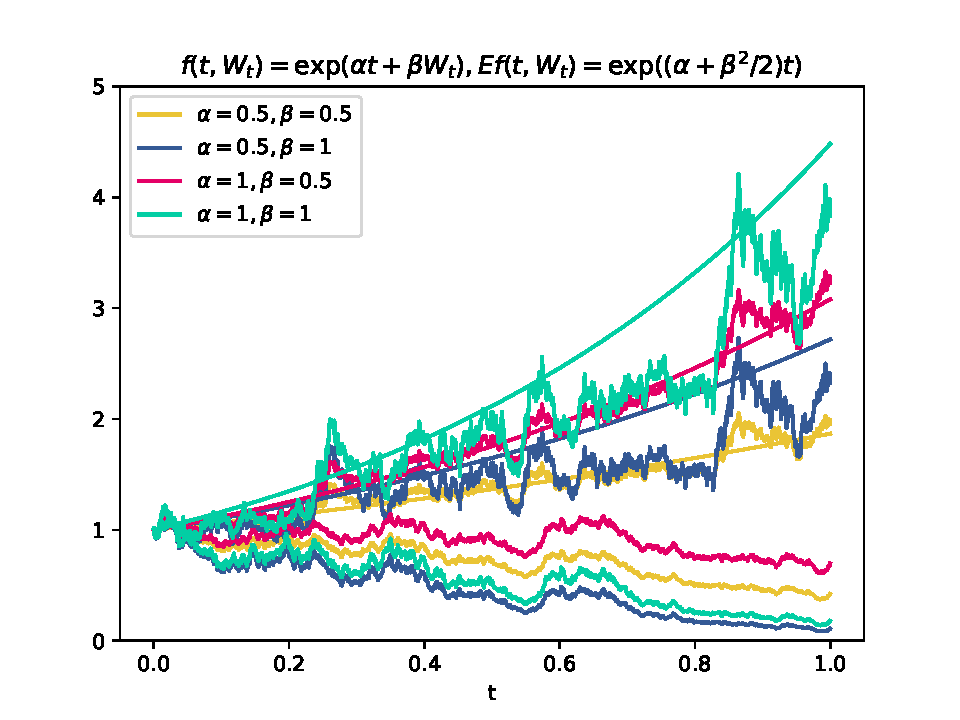
\includegraphics[width=\textwidth]{GBM}
        \caption{Graph of $f(t,W_t)$ and its expectation with different
        parameters}
        \label{fig:GBM}
    \end{figure}
\end{subproblem}

\problem
We can see from \cref{tab:diff} that the error tends to 0 as $N$ goes large.

\begin{margintable}
    \centering
    \begin{tabular}{cc}
        \toprule
        $k$ & error \\
        \midrule
        $2^{2}$ & $0.14513$\\
        $2^{4}$ & $0.26219$\\
        $2^{6}$ & $0.05478$\\
        $2^{8}$ & $0.04009$\\
        $2^{10}$ & $0.02272$\\
        \bottomrule
    \end{tabular}
    \caption{Difference Between It\^o and Stratonovich Integral}
    \label{tab:diff}
\end{margintable}

\problem
As we can see in \cref{fig:num}, in general,
% TODO Description

\begin{figure}[h]
    \centering
    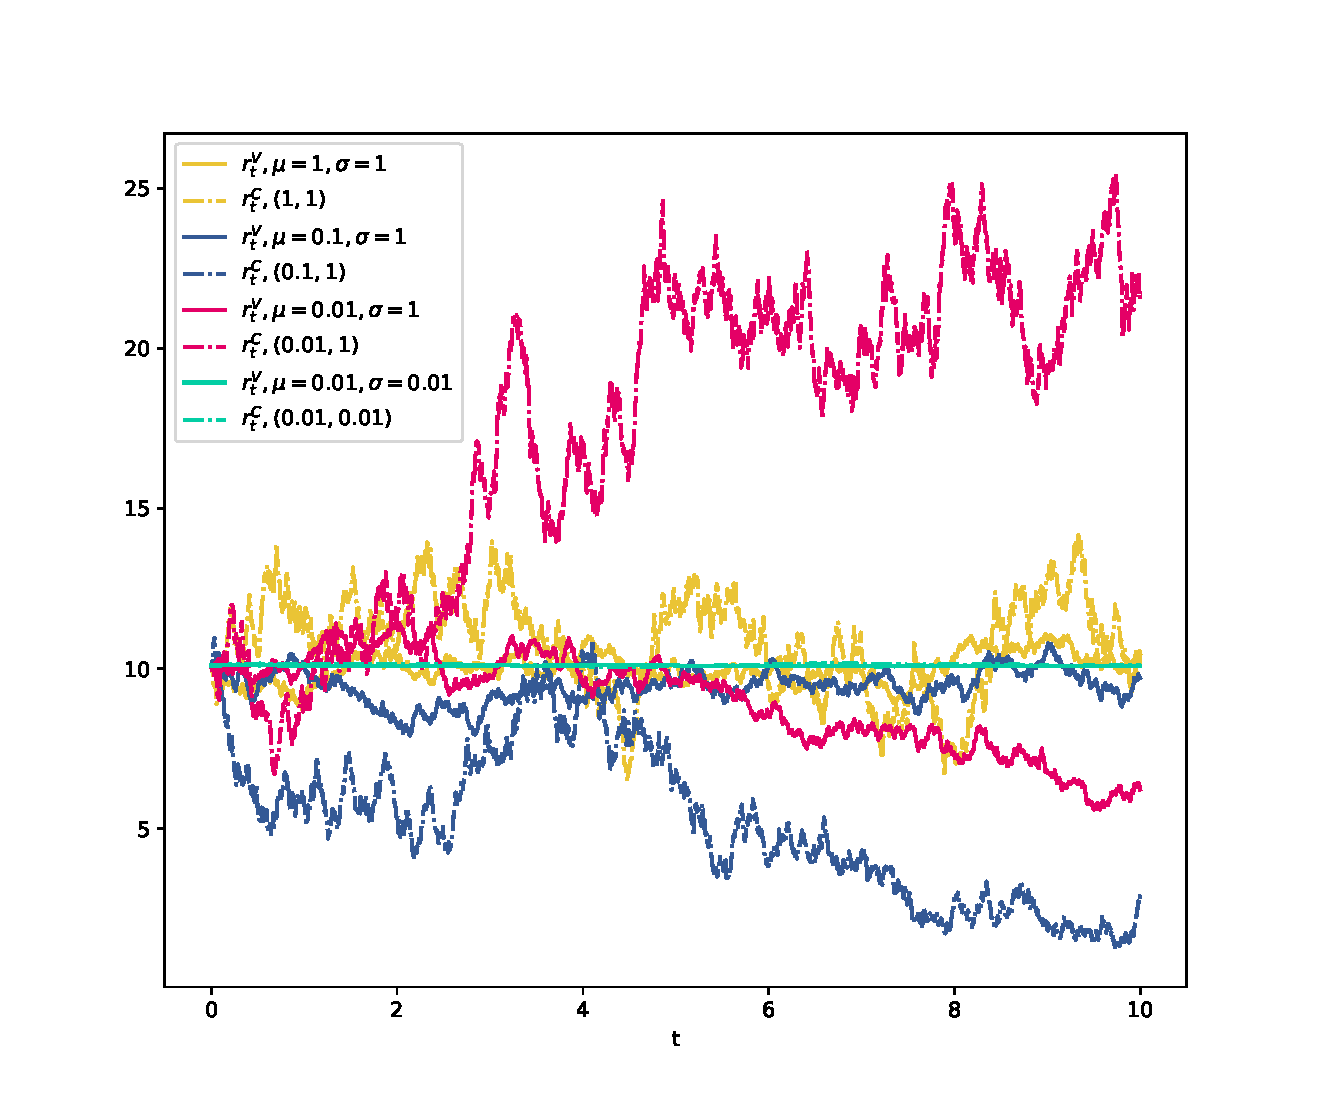
\includegraphics[width=\textwidth]{num}
    \caption{$r_t^V$ and $r_t^C$}
    \label{fig:num}
\end{figure}

\appendix
\section{Python Code}
\subsection{Code for Plotting $f(t,W_t)$}
\lstinputlisting[language=Python]{plot.py}
\subsection{Comparison of It\^o and Stratonovich}
\lstinputlisting[language=Python]{str-ito.py}
\subsection{Numerical Solution}
\lstinputlisting[language=Python]{numerical.py}